\documentclass{beamer}
\usepackage[english]{babel}
\usetheme{Warsaw}
\usepackage{pgfplots}
 

\pgfplotsset{
	compat=newest,
	xlabel near ticks,
	ylabel near ticks
}






\title[Animales]{II proyecto de Compiladores e Interpretes - Analizador L\'exico}
\subtitle[short subtitle]{Semestre: II}
\author{Integrante: Carlos Ad\'an Arguello Calder\'on}
\institute{Instituto Tecnol\'ogico de Costa Rica}
\date{\today}



\begin{document}

\begin{frame}
   \titlepage {}
\end{frame}

\begin{frame}

	\frametitle{\'Indice}
	\tableofcontents
	
	\section{Explicaci\'on general}
	\subsection{1-Proceso del scanning}
	
	\subsection{2-Herramienta de flex}
	
	\section{Slides del programa fuente}
	
	\section{Histograma de las cantidades de cada tipo de token encontrados en el fuente.}
	
	\section{Slides gr\'afico de las categor\'ias l\'exicas}
		
\end{frame}

\begin{frame}
	\frametitle{Explicaci\'on general-Proceso del scanning}
	
	\textbf{El proceso del scanning consiste en
		palabras b\'asicas consiste en realizar el análisis l\'exico de un programa determinado (en nuestro caso, el programa simple). Se lee el programa fuente como una secuencia de caract\'eres y reconoce unidades textuales "m\'as grandes" llamados tokens. }
	
	
	
\end{frame}
	
\begin{frame}
	\frametitle{Explicaci\'on general-Herramienta Flex}
	
	\textbf{Es una herramienta para la generación de esc\'eneres. En lugar de escribir un analizador de cero, sólo tiene que identificar el vocabulario de un idioma determinado (por ejemplo simple), escribir una especificación de patrones usando expresiones regulares (por ejemplo dígito [0-9]), y FLEX construirá un escáner para tú. FLEX se utiliza generalmente en la manera explicada aquí: }
	
	
\end{frame}


\begin{frame}
	\frametitle{Explicaci\'on general-Herramienta Flex}
	
	\textbf{Para poder crear un escaner tipo flex
		se debe tener un archivo.l que ese es el que
		se va a convertir en el escaner a utilizar, logico que en el archivo.l debemos tener todas las reglas y otras cosas, una vez teniendo eso debemos instalar flex si no lo tenemos instalado en SO ya una vez haciendo con el comando invocaremos al archivo.l para crear un archivo.c que ese sera el escaner a utilizar}
	
\end{frame}

\begin{frame}
	
	\frametitle{Fragmentito de codigo de preproceso-Algunos metodos utilizados en el Scanner}
	\textbf{
		TokenType getTokenType(FILE *filePtr) 
		int isExAcceptableChar(char);
		
		int isDelimiter(char);
		int isOtherOperators(char);
		int isStartRelationalOperator(char);
		
		
		void splitWords()
		void printWords()
		void printKeywords()
		void printNumbers()
		void printIdentifiers()
		
			

	}
		
\end{frame}
	
\begin{frame}
	\frametitle{Histograma}
	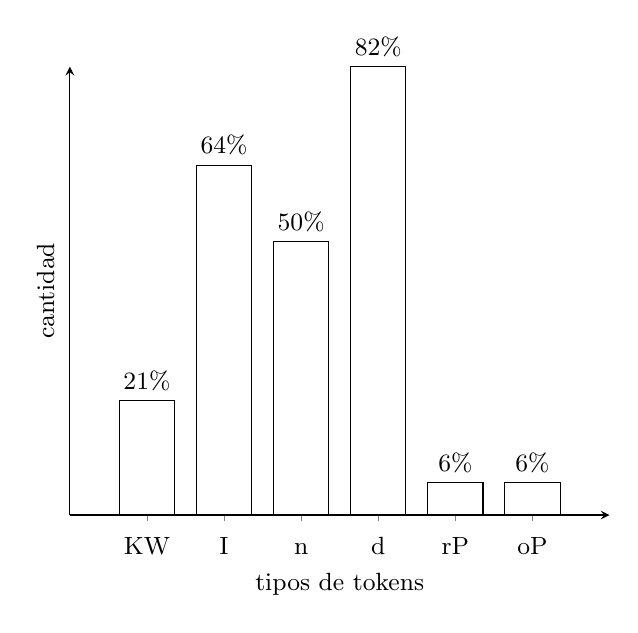
\begin{tikzpicture}[font=\small]
	\begin{axis}[
	ybar,
	bar width=20pt,
	xlabel={tipos de tokens},
	ylabel={cantidad},
	ymin=0,
	ytick=\empty,
	xtick=data,
	axis x line=bottom,
	axis y line=left,
	enlarge x limits=0.2,
	symbolic x coords={KW,I,n,d,rP,oP},
	xticklabel style={anchor=base,yshift=-\baselineskip},
	nodes near coords={\pgfmathprintnumber\pgfplotspointmeta\%}
	]
	\addplot[fill=white] coordinates {
		(KW,21)
		(I,64)
		(n,50)
		(d,82)
		(rP,6)
		(oP,6)
	};
	\end{axis}
	\end{tikzpicture}
\end{frame}

\begin{frame}
	
\end{frame}
	
\end{document}
